% Will grow up to be a journal paper at some point

\documentclass[10pt,a4paper]{article}
\usepackage[latin1]{inputenc}
\usepackage{amsmath}
\usepackage{amsthm}
\usepackage{amsfonts}
\usepackage{amssymb}
\usepackage{mathtools}
\usepackage{graphicx}
\usepackage{color}
\usepackage{hyperref}

% theorem environment
\newtheorem{prop}{Proposition}[section]
\newtheorem{theorem}{Theorem}[section]
\newtheorem{prop2}{Proposition}
\newtheorem{lem}{Lemma}
\newtheorem{ex}{Example}

% For algorithms
\usepackage{algorithm}
\usepackage{algorithmic}

% custom commands
\newcommand\at[2]{\left.#1\right|_{#2}} % the at differential sign
\newcommand\scalemath[2]{\scalebox{#1}{\mbox{\ensuremath{\displaystyle #2}}}} % scaling matrices

%% custom macros
\newcommand{\todo}{\textcolor{red}{TODO}} % TODO!
\newcommand{\kin}{\mathcal{T}} % used to denote inverse kinematics
\newcommand{\invKin}{\mathcal{T}^{-1}} % used to denote inverse kinematics

\newcommand{\joint}{q} % used to denote robot state in joint space
\newcommand{\state}{y} % denotes the generalized coordinates - joint space and velocity coordinates
\newcommand{\dmp}{s} % used to denote the dmp trajectory states
\newcommand{\error}{e} % difference between state and reference
\newcommand{\traj}{r} % used to denote the points on the trajectory to be tracked

\newcommand{\dist}{\epsilon} % denotes the disturbances acting on the rigid body dynamics
\newcommand{\linDist}{d} % denotes the disturbances on the LTV model

\newcommand{\sysInput}{u} % used to denote the system inputs
\newcommand{\linInput}{\tilde{u}} % denotes the LTV inputs
\newcommand{\trjInput}{\nu} % denotes the inputs on the trajectory


% % % % DMP terminology % % % %
\newcommand{\fullvec}{\psi} % full vector for state-ref-dmp-goal
\newcommand{\force}{f} % forcing term of the dmps
\newcommand{\phase}{x} % phase of the dmp
\newcommand{\weights}{w} % weights of the dmp
\newcommand{\basis}{\phi} % basis functions of the dmp as a matrix

% % % % ILC terminology % % % %
\newcommand{\qmatrix}{\Gamma} % denotes the filtering qmatrix term of Bristow et al.
\newcommand{\lmatrix}{L} % denotes the learning matrix of Bristow et al.

\newcommand{\observations}{\mathbf{y}} % used for the observed output
\newcommand{\dynamics}{f}
\newcommand{\dynamicsNominal}{f_{\mathrm{nom}}}
\newcommand{\policy}{\mathbf{\pi}}
\newcommand{\ValueFunction}{J}
\newcommand{\episode}{k} % used for episode number

\newcommand{\totalTime}{T} % total time duration 
\newcommand{\numSteps}{N} % total number of time steps
\newcommand{\numepisode}{K} % total number of episodes

\newcommand{\threshold}{\epsilon}
\newcommand{\alg}{\emph{wILC}}
\newcommand{\dataset}{E}

% Set the paths where all figures are taken from:
\graphicspath{{Pictures/}}
\mathtoolsset{showonlyrefs} 
\newcommand{\includesvg}[1]{%
% \executeiffilenewer{#1.svg}{#1.pdf}%
% {inkscape -z -D --file=#1.svg %
% --export-pdf=#1.pdf --export-latex}%
 \input{#1.pdf_tex}%
}

\author{Okan Ko\c c, Guilherme Maeda, Gerhard Neumann and Jan Peters}
\title{Optimal Striking Movement Representation \& Execution}
\begin{document}
\maketitle

\section{Introduction}\label{introduction}

% fill missing citations

Most reaching tasks in control and robotics can be phrased as \emph{tracking} problems, where the dynamical system needs to follow a certain predefined trajectory in order to reach the goal state. 

Robotic table tennis in particular consists of planning, generating and executing a series of such (episodic) single stroke trajectories. These trajectories need to be followed very closely with motor commands in practice, in order to return the ball to the desired positions. 

% maybe cite Jens' review paper
There have been many attempts in the reinforcement learning (RL) \cite{Sutton98} and control literature to learn robotic tasks directly. Value function based methods take advantage of duality to solve the Bellman's equation but suffer from the initial bias or representation in estimating the value function and do not scale well to high dimensions. Policy search methods directly solve the Bellman's equation in a parameterized policy space and can be much more effective in practice (in robotics). 
% maybe missing citation

% missing citations
Dynamic Motor Primitives (DMP) are a kind of kinematic policy representation that leverages the dynamical systems approach to modify the spring dynamics with a forcing term that enables it to mimic an executed trajectory. They include an internal phase or clock that ensures the convergence of the motor primitive to a goal state \cite{Ijspeert13}, \cite{Schaal07}. DMPs do not suffer from the curse of dimensionality as the number of parameters (weights) grow linearly with dimension. However, approximation and control errors in robotic platforms make the application of DMPs less useful in practice. Small changes to DMPs can often make them more useful.
% robotic platforms such as table tennis?

% Taken from the bimanual article
%They can be used to imitate or generate discrete and periodic trajectories, which can be modulated in various ways.

Motor primitives can work well with episodic policy search methods, such as POWER \cite{Kober08}, or REPS \cite{Peter10} that modify the weights based on the rewards in every episode. By adapting the DMP that was initialized with imitation learning, e.g. with kinesthetic teach-in, these model-free methods are able to achieve complex robotic tasks.
% complex tasks, such as?
% Katharina's papers come here maybe
% citation needed - also tone it down a notch?
% talk about PI2?

The research question that we tackle in this article consists of the following:

\begin{itemize}
\item How can we execute optimally hitting movement primitives either in table tennis or a similar reaching task, e.g. putting in golf.

\item More generally, when we have modelling inaccuracies, how should we modify a DMP $\dmp(t)$ such that the robot executes a desired hitting motion?
\end{itemize}

Iterative Learning Control (ILC) is a fundamental approach in control theory developed to track (time-varying) reference trajectories. It has been used successfully to follow trajectories under unknown repeating disturbances and model mismatch \cite{Bristow06}. In ILC, control inputs are adjusted at each episode in a feedforward fashion. The goal is to drive the deviations from the trajectory to zero. 

In this article, we combine Iterative Learning Control (ILC) with movement primitives by using ILC as a learning method to adapt the weights of the DMPs. This way we ensure a safe, reliant and robust way to track reference trajectories, with important applications in optimally hitting and striking motions. As opposed to model-free policy search approaches, we make full use of the known, albeit inexact, robot dynamics and inverse dynamics models, which helps us to quickly achieve the desired performance requirements. We validate the performance of the approach in two hitting tasks, and compare with existing episodic-RL approaches.
% nominal model instead of known, albeit inexact?

Finally our contributions can be summarized as follows:

\begin{itemize}
\item We form a link between the ILC literature and policy gradient based policy search approaches in Reinforcement Learning and develop a new algorithm that feeds on the strengths of both domains.
% really? does it feed on both?

\item We form the first coherent framework where some of the biggest advantages of using Dynamic Movement Primitives are leveraged in the feedforward update rule.

\item On the theoretical side, we come up with a new ILC algorithm \emph{wILC} that is shown to be stable and monotonically convergent.

\end{itemize}

In section~\ref{relatedWork} we mention related work especially the state-of-the-art approaches in hitting and reaching tasks. In section~\ref{problemStatement} we briefly review ILC and introduce our method in \ref{learningMPs}. In section~\ref{results} we evaluate our method in two robotic reaching tasks: putting motion in golf and the hitting motions in table tennis. We show that the method outperforms the state-of-the-art RL-based approaches REPS and PI2. Finally in section~\ref{conclusion} we discuss the strengths and weaknesses of our method and conclude with brief mentions of promising future research directions.

% Optimal Striking
% Talk about reinforcement learning
% Episodic setup - 'motor task consisting of a single stroke'
% Policy search methods
% DMPs
% Jens says : Dmps are a time-variant policy representation as they have an internal phase which corresponds to a clock with additional flexibility
% (e.g., for incorporating coupling effects, perceptual influences, etc.)
% Adapting DMPs
% Gait tracking
% Advantages of ILC Framework over Policy search 

\section{Related Work}\label{relatedWork}

% Policy search methods
Policy search methods that modify the parameters of a DMP appeared first with the \emph{POWER} algorithm \cite{Kober08}.
% is this true?

Iterative Learning Control started out in the 1980s with the work of Arimoto et al. \cite{Arimoto84} as one of the first to define the genre with the PD-type update law \cite{Bristow06}. Monotonic convergence and stability guarantees are of central importance for the practical usefulness of ILC algorithms. They are shown for example in \cite{Bristow06}, \cite{Norrloef02}, \cite{Lee97}, \cite{Longman2000}.
% check these refs

% ILC work - mention Angela's work
As an example of a more sophisticated method than the PD-type update laws, Schoellig et al. \cite{Schoellig12} applied a Kalman-filter based convex optimization rule in the framework of ILC and showed its performance in quadrocopter flight. 
% This work however lacks any guarantees of monotonic convergence

% DMPs using Iterative Learning Control
DMPs have been also combined in a bimanual robotics task with ILC \cite{Gams13} where force feedback is used to enable compliant interaction with objects in an unknown enviornment. ILC is here used to learn a coupling term between the two arm trajectories. ILC has not been used so far, as far as we know, to modify the weights of the motor primitives.
% used to modulate the DMP and learn ...


\section{Problem Statement}\label{problemStatement}

As stated in the introduction, our goal in this work is to track a given reference trajectory $\traj(t), \ 0 \leq t \leq T \ $ by applying the control inputs $\sysInput(t)$. We briefly review ILC in the next sections and show how learning can be represented within the movement primitives framework.

% this section probably belongs to a journal
\subsection{ILC Review}\label{ilcReview}

In this section we will first review some of the results from the Iterative Learning Control (ILC) literature \cite{Bristow06}. Consider the nonlinear robot dynamics of the form

\begin{equation}
\begin{aligned}
\ddot{\joint} &= \dynamics(\joint,\dot{\joint},\sysInput) \\
\ddot{\joint} &= M^{-1}(\joint)\{ \tau(\sysInput) - C(\joint,\dot{\joint})\dot{\joint} - G(\joint)\} + \dist(\joint,\dot{\joint})\\
\end{aligned}
\label{dynamics}
\end{equation}

\noindent where on the right hand side are the terms due to the rigid body dynamics model and $\dist(\joint,\dot{\joint})$ are the (unmodeled) disturbances that act on the robot, such as viscous friction, stiction, etc. This system can be linearized around a given joint space trajectory $\traj(t), \ 0 \leq t \leq T$ with nominal inputs $\nu(t)$~\footnote{Nominal inputs $\sysInput_{\mathrm{IDM}} = \nu(t)$ can be calculated using the inverse dynamics model.} to obtain the following linear time varying (LTV) representation

\begin{equation}
\begin{aligned}
\dot{\error} = A(t)\error(t) + B(t)\linInput(t) + \linDist(t,\sysInput)
\end{aligned}
\label{LTV}
\end{equation}

\noindent where $\error(t) = \state(t) - \traj(t)$, $\state = [\joint,\dot{\joint}]^{\mathrm{T}}$, $\linInput(t) = \sysInput(t) - \trjInput(t)$ and the time varying matrices are

\begin{equation}
\begin{aligned}
A(t) &= \at{\frac{\partial{\dynamics}}{\partial{\state}}}{(\traj(t),\trjInput(t))} \\
B(t) &= \at{\frac{\partial{\dynamics}}{\partial{\sysInput}}}{(\traj(t),\trjInput(t))}
\end{aligned}
\label{LTVmatrices}
\end{equation}

\noindent In \eqref{LTV} the additional term $\linDist(t,\sysInput)$ are due to the disturbances and the effects of the linearization. We can discretize (\ref{LTV}-\ref{LTVmatrices}) with step size $\Delta t$, $N = T/\Delta$ and step index $j = 1, \ldots, N$ to get the following discrete linear system

\begin{equation}
\begin{aligned}
\error(j+1) = A^{D}(j)\error(j) + B^{D}(j)\linInput(j) + \linDist(j, \sysInput(1), \ldots, \sysInput(j))
\end{aligned}
\label{discreteLTV}
\end{equation}

\noindent Here $A^D$ and $B^D$ are the discretizations of \eqref{LTVmatrices} and can be calculated using the following trick \cite{Schoellig12}

\begin{equation}
\begin{aligned}
\exp^{h
\left[
\scalemath{0.5}{
\begin{array}{c|c}
A(j) & B(j) \\ \hline
0 & 0
\end{array}}\right]}
&= 
\left[
\begin{array}{c|c}
A^{D}(j) & B^{D}(j) \\ \hline
0 & I
\end{array}\right] 
\end{aligned}
\label{discreteMatrices}
\end{equation}

\noindent We can stack these matrices together to get the following lifted-vector representation \cite{Bristow06}, \cite{Schoellig12}

\begin{equation}
\begin{aligned}
\error_L &= F\sysInput_L + \linDist_L \\
\end{aligned}
\label{liftedLTV}
\end{equation}

\noindent where the submatrices of $F$ are

\begin{equation*}
\begin{aligned}
F_{(i,j)} &= \left \{
\begin{array}{cc}
A^{D}(i-1)\ldots A^{D}(j)B^{D}(j-1), & j < i \\ 
B^{D}(j-1), & j = i \\
0, & j > i 
\end{array} \right.
\end{aligned}
\end{equation*}

\noindent Using this \emph{input-to-output matrix} $F$ we can analyze the effects of the ILC's feedforward input $\sysInput_L = [\linInput(1), \sysInput(2), \ldots, \linInput(\numSteps)]^{\mathrm{T}}$ on the errors $\error_L = [\error(1), \error(2),\ldots,\error(\numSteps)]^{\mathrm{T}}$ using ILC terminology.

The cost functional as the optimality criterion

\begin{equation}
\begin{aligned}
\ValueFunction(\policy) &= \int_{0}^{T} (\state - \traj)^{\mathrm{T}}Q(\state - \traj) + \linInput^{\mathrm{T}}R\linInput \ \mathrm{d}t + (\state_T-\traj_T)^{\mathrm{T}}Q_{T}(\state_T-\traj_T)
\end{aligned}
\label{cost}
\end{equation}

\noindent can be equally discretized and stacked in lifted vector form

\begin{equation}
\begin{aligned}
\ValueFunction_L &= \error_L^{\mathrm{T}}Q_L\error_L + \sysInput_L^{\mathrm{T}}R_L\sysInput_L
\end{aligned}
\label{costFunctional}
\end{equation}

\noindent where $Q_L, R_L \in \mathbb{R}^{N \times N}$ are of the following form

\begin{equation*}
\begin{aligned}
 Q_L &= 
 \begin{bmatrix}
  Q & 0 & \cdots & 0 \\
  0 & Q & \cdots & 0 \\
  \vdots  & \vdots  & \ddots & \vdots  \\
  0 & 0 & \cdots & Q_T
 \end{bmatrix} \\
 R_L &= 
  \begin{bmatrix}
   R & 0 & \cdots & 0 \\
   0 & R & \cdots & 0 \\
   \vdots  & \vdots  & \ddots & \vdots  \\
   0 & 0 & \cdots & R
  \end{bmatrix}
\end{aligned}
\end{equation*}

\noindent Most ILC update laws can be put in the following form

\begin{equation}
\begin{aligned}
\sysInput_{k+1} = \qmatrix(\sysInput_{k} - \lmatrix\error_{k})
\end{aligned}
\label{ILCupdateForm}
\end{equation}

\noindent \emph{Gradient descent} of \eqref{costFunctional} is also in this form

\begin{equation}
\begin{aligned}
\sysInput_{k+1} &= \sysInput_k - \frac{\beta_k}{2} \at{\frac{\partial{\ValueFunction_L}}{\partial{\sysInput_L}}}{\sysInput_k} \\
\frac{1}{2}\frac{\partial{\ValueFunction_L}}{\partial{\sysInput_L}} &= \frac{\partial{\error_L}}{\partial{\sysInput_L}}Q_L\error_L + R_L\sysInput_L \\
\sysInput_{k+1} &= (I - \beta_kR_L)\sysInput_k - \beta_k\frac{\partial{\error_L}}{\partial{\sysInput_L}}Q_L\error_k
\end{aligned}
\label{ILCgradientDescentEq1}
\end{equation}

\noindent If the disturbances are repeating every iteration, i.e. $\frac{\partial{\linDist_L}}{\partial{\sysInput_L}} = 0$, using \eqref{liftedLTV}, we can rewrite \eqref{ILCgradientDescentEq1} as

\begin{equation}
\begin{aligned}
\sysInput_{k+1} = (I - \beta_kR_L)\sysInput_k - \beta_kF^\mathrm{T}Q_L\error_k
\end{aligned}
\label{ILCgradientDescentEq2}
\end{equation}

\noindent where $\qmatrix = I - \beta_kR_L$ and $\lmatrix = (I - \beta_kR_L)^{-1}\beta_kF^\mathrm{T}Q_L$. This gradient-descent ILC converges linearly to $\error_L = 0$ as $k \to \infty$, if $\beta_k$ is kept sufficiently small \cite{Nocedal99}.
% check the citation and the assumptions

In the ideal case, if $\frac{\partial{\linDist_L}}{\partial{\sysInput_L}} = 0$, taking $R_L = 0$, the following \emph{Newton's method} based ILC~\footnote{Here we are using the column-vector version of matrix calculus where the chain rule for vectors is written as $\frac{\partial\mathbf{y}}{\partial\mathbf{x}} = \frac{\partial\mathbf{z}}{\partial\mathbf{x}}\frac{\partial\mathbf{y}}{\partial\mathbf{z}}$.}

\begin{equation}
\begin{aligned}
\sysInput_{k+1} &= \sysInput_k - \beta_k\Big(\frac{\partial^{2}\ValueFunction_L}{\partial\sysInput^{2}_L}\Big)^{-1}\at{\frac{\partial{\ValueFunction_L}}{\partial{\sysInput_L}}}{\sysInput_k} \\
\frac{\partial^{2}\ValueFunction_L}{\partial\sysInput^{2}_L} &= \frac{\partial}{\partial\sysInput_L}\{F^{\mathrm{T}}Q_L\error_L\} = F^{\mathrm{T}}Q_LF \\
\sysInput_{k+1} &= \sysInput_k - \beta_kF^{\dagger}\error_k
\end{aligned}
\label{ILCnewtonsMethod}
\end{equation}

\noindent is guaranteed to converge in one step if $\beta_k = 1$, independent of the previously applied input. However it suffers from numerical stability due to the inversion of $F$, and will be prone to diverge in practical applications \cite{Bristow06}. Keeping $R_L \neq 0$ turns \eqref{ILCnewtonsMethod} into a \emph{Levenberg-Marquardt} \cite{Nocedal99} type ILC algorithm for \eqref{cost} with $R = 0$, giving additional stability

\begin{equation}
\begin{aligned}
\sysInput_{k+1} &= \sysInput_k - \beta_k(F^{\mathrm{T}}Q_LF + R_L)^{-1}F^{\mathrm{T}}Q_L\error_k
\end{aligned}
\label{ILClevenbergMarquardt}
\end{equation}

\noindent assuming $\beta_k(F^{\mathrm{T}}Q_LF + R_L)^{-1}R_L \approx 0$.
% check the citation and the assumptions

%\todo I don't like the qbar notation
%\todo Stability and monotonic convergence.\\
%\todo Estimate $F_{est}(\error_1, \error_2, \ldots, \error_k) \neq F$.\\
%\todo Line search for $\beta_k$.\\
%\todo Guarantee decrease by using 'descent direction'
%\todo Noncausal ILC. 
%\todo Monotonic convergence and stability
%\todo Is Angela's method a Newton-Raphson based approach?
%\todo Is an iteration-based update law possible?

\subsubsection{Stability analysis}

\subsection{Learning the Motor Primitive Parameters}\label{learningMPs}

Sometimes for safety reasons~\footnote{For instance, when interacting with external objects or under unforeseen perturbations \cite{Schaal07}} a \emph{low-gain} feedback law operating on the inputs may be fine-tuned to be compliant or one may not even be allowed to modify the low-level controller of the industrial robot \cite{Longman2000}. In such cases, it is not possible to modify the input signals $\sysInput_L$ directly. Instead one can modify the reference trajectories that are provided to the low-level controllers. It can be shown that this is an equivalent approach to modifying the feedforward control inputs \cite{Bristow06}.

In this work we focus on modifying the parameters or the weights of the dynamic motor primitives (DMP), which acts as a \emph{kinematic policy} $\dmp(t) = [\joint_{\text{des}},\dot{\joint}_{\text{des}}]^{\mathrm{T}}$. For a linear time-varying system under a given linear feedback law $\linInput = -K_u(\state - \dmp)$ we consider the following transition dynamics

\begin{equation}
\begin{aligned}
 \dot{\fullvec} = 
 \begin{bmatrix}
  \dot{\state} \\
  \dot{\traj} \\
  \dot{\dmp} \\
  \dot{g}
 \end{bmatrix} = 
 \underbrace{\begin{bmatrix}
  A_q(t) - B_q(t)K_u & 0 & B_q(t)K_u & 0 \\
  0 & 0 & 0 & \nu(t) \\
  0  & 0  & A_s & A_g  \\
  0 & 0 & 0 & 0
 \end{bmatrix}}_{A_{\fullvec}}
 \begin{bmatrix}
   \state \\
   \traj \\
   \dmp \\
   g
  \end{bmatrix} +
  \underbrace{\begin{bmatrix}
    0 \\
    0 \\
    \basis(\phase) \\
    0
   \end{bmatrix}}_{B_{\fullvec}} \weights + \linDist(t,\weights)
\end{aligned}
\label{fullTransition}
\end{equation}

where the phase $\phase$ evolves according to

\begin{equation}
\dot{\phase} = -\tau\alpha\phase
\label{phase}
\end{equation}

The constants $\tau$ and $\alpha$ determine the scaling and settling time respectively. $A_s$ and $A_g$ matrices include the spring constants that drive the DMP to the goal state $g$.
% this needs to be rephrased perhaps.

If we introduce for this enlarged vector $\fullvec$ the following cost functional

\begin{equation}
\begin{aligned}
J(\weights) &= \int_{0}^{T} (\state - \traj)^{\mathrm{T}}Q(\state - \traj) + \weights^{\mathrm{T}}R_w\weights \ \mathrm{d}t +  (\state_T-\traj_T)^{\mathrm{T}}Q_{T}(\state_T-\traj_T) 
\end{aligned}
\label{cost2}
\end{equation}

we can apply a weight-update form of the ILC update law \eqref{ILCupdateForm}

\begin{equation}
\begin{aligned}
\weights_{k+1} = \qmatrix(\weights_{k} - \lmatrix\error_{k})
\end{aligned}
\label{ILCupdateFormWeights}
\end{equation}

To do this, we discretize \eqref{cost2} as in \eqref{costFunctional}

\begin{equation}
\begin{aligned}
\ValueFunction_L &= \error_L^{\mathrm{T}}Q_L\error_L + \weights^{\mathrm{T}}R_w\weights
\end{aligned}
\label{costFunctionalWeights}
\end{equation}

where the lifted output $\error_L$ can be written as the lifted output matrix $C_L$ times the lifted state vector $\fullvec_L$

\begin{equation}
\begin{aligned}
\error_L &= C_L \fullvec_L \\
C_L &= 
  \begin{bmatrix}
   C & 0 & \cdots & 0 \\
   0 & C & \cdots & 0 \\
   \vdots  & \vdots  & \ddots & \vdots  \\
   0 & 0 & \cdots & C
  \end{bmatrix} \\
C &= \begin{bmatrix}
  I_{2n} & -I_{2n} & 0_{2n} & 0
 \end{bmatrix}
\end{aligned}
\label{outputWeights}
\end{equation}

Notice that now the weighting matrix $R_w \in \mathbb{R}^{m \times m}$ where $m$ is the number of basis functions used in the controls matrix $B_{\fullvec}$ or equivalently $m = \text{rank}(B_{\fullvec})$.

Gradient descent of \eqref{costFunctionalWeights} can be put in this form \eqref{ILCupdateFormWeights}

\begin{equation}
\begin{aligned}
\weights_{k+1} &= \weights_k - \frac{\beta_k}{2} \at{\frac{\partial{\ValueFunction_L}}{\partial{\weights}}}{\weights_k} \\
\frac{1}{2}\frac{\partial{\ValueFunction_L}}{\partial{\weights}} &= \frac{\partial{\error_L}}{\partial{\weights}}Q_L\error_L + R_{\weights}\weights \\
\weights_{k+1} &= (I - \beta_kR_{\weights})\weights_k - \beta_k\frac{\partial{\fullvec_L}}{\partial{\weights}}\at{\frac{\partial{\error_L}}{\partial{\fullvec_L}}}{\fullvec_k}Q_L\error_k
\end{aligned}
\label{ILCgradientDescentWeights}
\end{equation}

If the disturbances are repeating every iteration, i.e. $\frac{\partial{\linDist_L}}{\partial{\weights}} = 0$, using \eqref{liftedLTV}, we can rewrite \eqref{ILCgradientDescentWeights} as

\begin{equation}
\begin{aligned}
\weights_{k+1} = (I - \beta_kR_{\weights})\weights_k - \beta_kF_{\weights}^\mathrm{T}Q_L\error_k
\end{aligned}
\label{ILCgradientDescentWeights2}
\end{equation}

where the \emph{weight-to-output matrix} $F_{\weights}$ is defined as

\begin{equation}
\begin{aligned}
\error_L &= F_{\weights}\weights + \linDist_L \\
\frac{\partial{\error_L}}{\partial{\weights}} &= F_{\weights}^{\mathrm{T}} = \frac{\partial{\fullvec_L}}{\partial{\weights}}C_L^{\mathrm{T}} = 1_{m\times Nm}\tilde{F}_{\weights}^{\mathrm{T}}C_L^{\mathrm{T}} \\
(\tilde{F}_{\weights})_{(i,j)} &= \left \{
\begin{array}{cc}
A^{D}_{\fullvec}(i-1)\ldots A^{D}_{\fullvec}(j)B^{D}_{\fullvec}(j-1), & j < i \\ 
B^{D}_{\fullvec}(j-1), & j = i \\
0, & j > i 
\end{array} \right. \\
1_{m\times Nm} &= \begin{bmatrix}
  I_{m} & I_{m} & \ldots & I_{m}
 \end{bmatrix}
\end{aligned}
\label{weightToOutputMatrix}
\end{equation}

The matrix $1_{m\times Nm}$ appears in \eqref{weightToOutputMatrix} because the weight vector $\weights$ is not dynamic, as opposed to the feedback inputs $\linInput$.

% check numerical optimization book - is this really LM?

The following \emph{Levenberg-Marquardt} (LM) type ILC law updates the weights

\begin{equation}
\begin{aligned}
\weights_{k+1} &= \weights_k - \beta_k\Big(\frac{\partial^{2}\ValueFunction_L}{\partial\weights^{2}}\Big)^{-1}\at{\frac{\partial{\ValueFunction_L}}{\partial{\weights}}}{\weights_k} \\
\frac{\partial^{2}\ValueFunction_L}{\partial\weights^{2}} &= \frac{\partial}{\partial\weights}\{F_{\weights}^{\mathrm{T}}Q_L\error_L + R_{\weights}\weights\} = F_{\weights}^{\mathrm{T}}Q_LF_{\weights} + R_{\weights} \\
\weights_{k+1} &= \weights_k - \beta_k(F_{\weights}^{\mathrm{T}}Q_LF_{\weights} + R_{\weights})^{-1}F_{\weights}^{\mathrm{T}}Q_L\error_k
\end{aligned}
\label{ILCWeightsNewtonsMethod}
\end{equation}

assuming again that $\beta_k(F_{\weights}^{\mathrm{T}}Q_LF_{\weights} + R_{\weights})^{-1}R_{\weights} \approx 0$. Expanding the terms in the weight-to-output matrix $F_{\weights}$

\begin{equation}
\begin{aligned}
F_{\weights} &= \begin{bmatrix}
  0_{2n \times m} & B_{\joint}(2)K_{\sysInput}\basis_{1} & \ldots
 \end{bmatrix}^{\mathrm{T}}
\end{aligned}
\label{weightToOutputMatrixExpanded}
\end{equation}

we can rewrite \eqref{ILCWeightsNewtonsMethod} as

% show this properly!
\begin{equation}
\begin{aligned}
\weights_{k+1} &= \weights_k - \beta_k(\Phi^{\mathrm{T}}W(t)\Phi + R_{\weights})^{-1}\Phi^{\mathrm{T}}W(t)\error_k \\
\Phi &= \begin{bmatrix}
  \basis_1 & \basis_2 & \ldots & \basis_N
 \end{bmatrix}
\end{aligned}
\label{ILCWeightedRidgeRegression}
\end{equation}

% definitely reference needed for regression based weight update
Notice the connection of \eqref{ILCWeightedRidgeRegression} with the weight update law based on ridge regression where the weighting matrix is the identity matrix. In this case the model-based assumptions of our approach appear in the form of a nondiagonal weighting matrix, i.e. we perform the regression update using a different metric.
% model based update-law

\subsubsection{Algorithm}

We use the update law derived in \eqref{ILCWeightedRidgeRegression} in our algorithm, given in Algorithm~\ref{alg1}. We initialize the algorithm $\alg$ with the necessary weighting and transition matrices. The transition matrix $A_{\fullvec}$ is derived by linearizing the nominal robot dynamics around the given reference trajectory $r$. Nominal inputs $\nu$ are acquired using the inverse dynamics model. Weights of the DMPs are initialized for each degree of freedom using weighted regression on the reference trajectory.

% notice the stability of the approach compared to iLQR methods where the reference trajectory and the nominal inputs are varying at each iteration, contributing to the source of the instabilities often encountered in such iterative linear optimal control approaches.

\begin{algorithm}[tb]
   \caption{\alg}
   \label{alg1}
\begin{algorithmic}
   \STATE {\bfseries Input:} $\threshold > 0$, $\beta > 0$, $Q_L, R_{\weights} \succeq 0$, $A_{\fullvec}$, $\ \traj = \{\traj_0, \traj_1, \ldots, \traj_N \}$, $\ \nu = \sysInput_{\mathrm{IDM}} = \{\nu_0, \nu_1, \ldots, \nu_N \}$
   \STATE Initialize $k = 1$, $\dmp(\weights) = \dmp(\weights_0)$, $\beta_k = \beta$
   \REPEAT 
 	   \STATE Run controller $\ddot{\joint} \leftarrow \dynamics(\joint,\dot{\joint},\sysInput)$ %\sysInput = \nu - K_{\sysInput}(\state - \dmp(\weights)))$
 	   \STATE Observe $\error = \state - \traj$
 	   \STATE Compute $\ValueFunction_k$ = $\error_L^{\mathrm{T}}Q_L\error_L + \weights^{\mathrm{T}}R_w\weights$
 	   \STATE Form $W(t)$ from $A_{\fullvec}$, $Q_L$
 	   \STATE Update weights $\weights \leftarrow \weights - \beta_k(\Phi^{\mathrm{T}}W(t)\Phi + R_{\weights})^{-1}\Phi^{\mathrm{T}}W(t)\error_L$
 	   \STATE $k \leftarrow k + 1$
   \UNTIL{$\ValueFunction_k < \threshold$}
\end{algorithmic}
\end{algorithm}

\subsubsection{Stability analysis}

\section{Results}\label{results}

In this section, we demonstrate the effectiveness of the algorithm presented in Section 2.3 in the context of movement primitive learning for optimally striking motions. We consider two hitting tasks: putting in golf and returning the ball with the racket in table tennis. In each task trajectories and the movement primitives are assigned in joint space. 
% underactuated swing-up belongs to putting-like dynamics problems?

\subsection{Putting}

Putting is a simple and natural domain for ILC algorithms, because it allows a robot to apply ILC to control few degrees of freedom (typically the end joint) while having the dynamics of the other joints act as disturbances. This kind of learning can act as a scalable interface to more complex hitting tasks in the full-joint space.

\subsection{Table Tennis}

As a second and more complex task, we consider table tennis where we are interested in generating and executing accurate ball-hitting motions. The racket is mounted on the end-effector of the 7 degree of freedom (DoF) WAM Barrett arm as can be seen in Figure~\ref{barrettArm}. A fixed ball-thrower is available to throw balls accurately to a fixed position in cartesian space, using which 7 joint-space reference trajectories are calculated. These trajectories guide the robot to the desired racket position and orientation so that the incoming ball will be hit precisely at the desired time and position with the desired velocity. 

\begin{figure}
\center
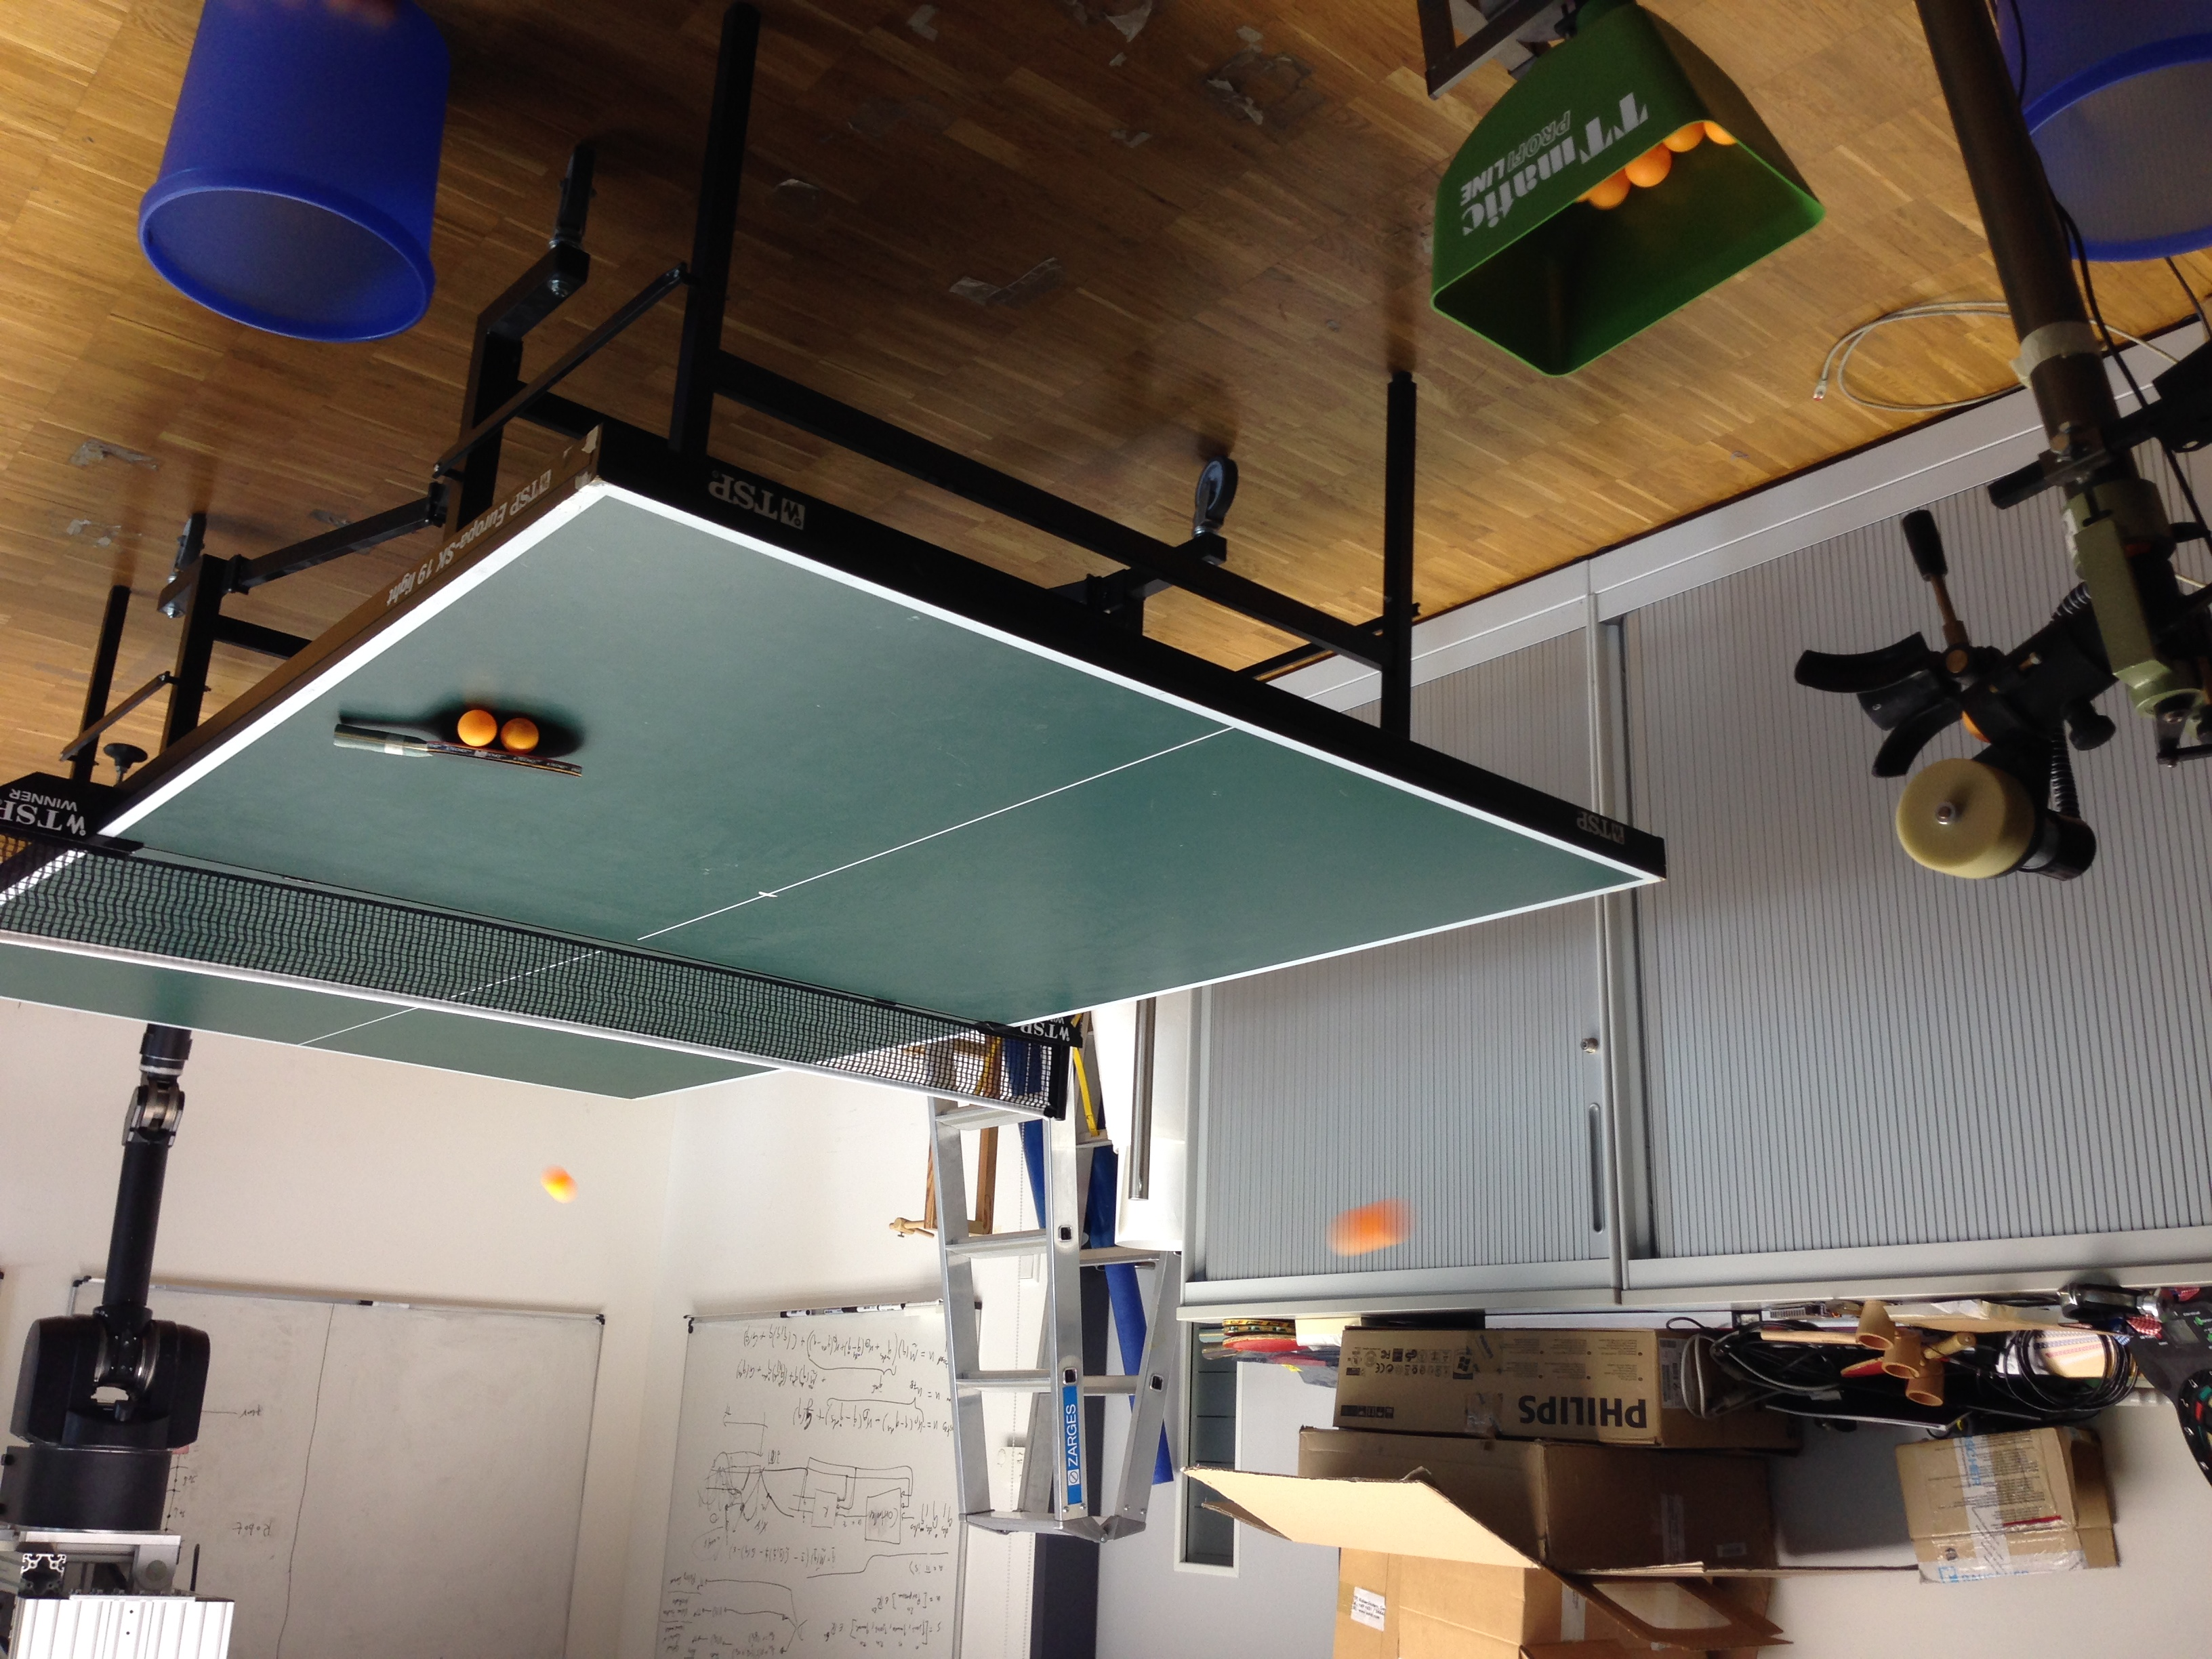
\includegraphics[scale=0.05, angle= 180]{ballgun.jpg}			
\caption{Robotic table tennis setup with the ballgun throwing balls to the robot}
\label{barrettArm}
\end{figure}

The attached video shows the improvement achieved after using $\alg$. The convergence of the algorithm can be seen in Figure 2 and some examples of the generated trajectories in the joint are given in Figure 3. Comparisons to episodic-RL algorithms REPS and PI2 show the advantages, especially the speed and accuracy of the proposed method over them.

\section{Conclusion}\label{conclusion}

In this paper we presented a novel Iterative Learning Control algorithm that tracks trajectories by adapting the weights of dynamic movement primitives. Weights are adapted after each episode by using a Levenberg-Marquardt type update rule on the deviations from the reference trajectories. These reference trajectories are generated in the joint space of the robot and enable the robot to execute optimally striking motions. We show two example experiments where we evaluate the performance of the approach in putting in golf and in ball-hitting with a racket in robotic table tennis. 

Reference trajectories are used in our approach only as a way to end up at the desired hitting states within the desired time frame. We are currently evaluating new ways within the optimal control perspective where the dependence on this sometimes arbitrary reference trajectory diminishes over the iteration domain, as the robot gets more confident in the hitting motion.

Finally a natural extension of the DMP representation is the generalization ability of these differential equations to different hitting motions and trajectories. We think that with our method, a stochastic approach to guide exploration is missing, and it is this that restricts the generalization ability of the proposed algorithm. By extending our framework to include the Probabilistic Movement Primitives~\cite{Paraschos13} we hope to increase the generalization ability and leverage the probabilistic logic of these movement primitives.

\bibliographystyle{plain}
%\bibliographystyle{./IEEEtran}
%\bibliography{./IEEEabrv,./iros2015Ref}
\bibliography{./iros2015Ref}

\end{document}
